% !TeX encoding = UTF-8
% !TeX document-id = {856115b6-76ae-40a0-94c7-827233f04a27}
\documentclass[13pt,a4paper, listof=entryprefix, bibliography=totocnumbered,toc=listofnumbered,lof=listofnumbered]{scrartcl}
																			%toc=listofnumbered
% WICHTIG!!!
% Pseudokommentar um pdflatex zu erlauben andere Programme zu nutzen z.B. gnuplot
% !TeX TXS-program:compile = txs:///pdflatex/[--shell-escape] | txs:///makeindex | txs:///biber | txs:///pdflatex/[--shell-escape]

\usepackage[normalem]{ulem}
\usepackage[ngerman]{babel}
\usepackage{romannum}
\usepackage[utf8]{inputenc}

%Paket fuer einheitlichen Schriftsatz Times Roman
\usepackage{mathptmx}

%Paket wurde eingefügt, damit die Trennung auch bei Umlauten korrekt erfolgt
\usepackage[T1] {fontenc} 
%sollte ein Wort trotzdem mal nicht richtig getrennt werden, kann dies durch
%\hyphenation{Durch-füh-rung} %manuel getrennt werden.


\usepackage{amsmath}
\usepackage{booktabs}
\usepackage{nccmath}
\usepackage{amsfonts}
\usepackage{amssymb}
\usepackage{adjustbox}
\usepackage{graphicx}
\usepackage{fancyhdr}
\usepackage{array}
\usepackage{tabularx}
\usepackage{geometry}
\usepackage{setspace}
\usepackage[right]{eurosym}
\usepackage[printonlyused]{acronym}
\usepackage{subfig}
\usepackage{floatflt}
\usepackage[usenames,dvipsnames]{color}
\usepackage{colortbl}
\usepackage{xcolor}
\usepackage{paralist}
\usepackage{array}
%\usepackage{titlesec}
\usepackage{parskip}
\usepackage{picinpar}
\usepackage[pdfpagelabels=true]{hyperref}
\usepackage{listings}
\usepackage{csquotes}
\usepackage{url}
\usepackage{float}
\usepackage{pgfplots}
\usepackage[nonumberlist, nogroupskip]{glossaries}
\usepackage{eurosym}
\usepackage{textcomp}
 
\usepackage{ltablex}

\usepackage{lscape}
\usepackage{verbatim}
\usepackage{enumitem} 
\usepackage{tex/ampl}
\usepackage{multirow}
\setitemize{leftmargin=*}
%\usepackage{pdflscape}
\usepackage[miktex]{gnuplottex}
% Wird benötigt, damit die Tabelle beim Spaltentyp X die gesamte Seitenbreite verwendet. Ist unter anderem bei Tabellen in der Parameter definiert werden hilfreich.
\keepXColumns




%Wird zur Darstellung von Algorithmen benötigt
\usepackage{algorithm}
\usepackage{algorithmic}

\floatname{algorithm}{Algorithmus}
\floatname{List of Algorithms}{Algorithmen}
\captionsetup[algorithm]{justification=raggedright,singlelinecheck=false}

% Indizes
\index{Algorithmus -- Pseudocode}
\index{Optimierungsproblem -- Definition}


% Stichwortverzeichnis
\usepackage[nonewpage]{imakeidx}
\makeindex[intoc=false, title=, options=-g -s tex/_index \%.idx]


%-----------------------------------------------------------------------------------
% Bibilothek
%-----------------------------------------------------------------------------------
% Einbinden des BibLateX paketes mit Ausgabeeinstellungen							   
\usepackage[
style=alphabetic,          % Zitierstil
maxbibnames=50,            % alle Autorennamen anzeigen
maxcitenames=4,            % maximale Namen, die im Kürzel angezeigt werden
autocite=inline,           % regelt Aussehen für \autocite (inline=\parancite)
block=space,               % kleiner horizontaler Platz zwischen den Feldern
backref=false,             % Keine Angaben auf welchen Seiten die Quelle referenziert ist
% backrefstyle=three+,       % fasst Seiten zusammen, z.B. S. 2f, 6ff, 7-10
% date=short,                % Datumsformat
backend = biber,           % Backnend für Aufbereitung
doi=false,		%Keine Ausgabe des DOI
isbn=false		% Keine Ausbage der ISBN
]{biblatex}

%Doppelunkt nach Autorennamen
\renewcommand*{\labelnamepunct}{\addcolon\addspace}

%Zusätzliche für Umbrüche für Kleinbuchstaben z.B. in URLs
\appto\textitBreaks{\do\a\do\b\do\c\do\d\do\e\do\f\do\g\do\h\do\i\do\j
	\do\k\do\l\do\m\do\n\do\o\do\p\do\q\do\r\do\s\do\t\do\u\do\v\do\w
	\do\x\do\y\do\z}



\newcounter{verzeichnis}
\setcounter{verzeichnis}{1}

%zur Verwendung von TikZ
\usepackage{tikz}
\usepackage{tikz-qtree, tikz-qtree-compat}
\usetikzlibrary{patterns}
%\usepackage[justification=RaggedRight,singlelinecheck=false]{caption}
\usetikzlibrary{positioning,calc}
\usetikzlibrary{snakes,arrows,shapes,automata,positioning}
\usetikzlibrary{decorations,decorations.pathmorphing,decorations.markings,trees,arrows}
\usetikzlibrary{shapes.geometric}
\usetikzlibrary{arrows.meta}
\usetikzlibrary{graphs,quotes,angles, babel}


%Abstände der Einträge
\setlength{\bibitemsep}{1em}     % Abstand zwischen den Literaturangaben
\setlength{\bibhang}{2em}        % Einzug nach jeweils erster Zeile

% Kürzel soll vier Buchstaben der Autoren enthalten statt drei
\DeclareLabelalphaTemplate{
	\labelelement{
		\field[final]{shorthand}
		\field{label}
		\field[strwidth=4,strside=left,ifnames=1]{labelname}
		\field[strwidth=2,strside=left,ifnames=2]{labelname}
		\field[strwidth=1,strside=left]{labelname}
	}
	\labelelement{
		\field[strwidth=2,strside=right]{year}
	}
}

% Bibliothek der Quellen
\bibliography{tex/biblatex.bib}
\label{bib}


% --------------------------------------------------------------------------------
% Einstellung für Listings
% --------------------------------------------------------------------------------
\lstset{basicstyle=\footnotesize, captionpos=b, breaklines=true, showstringspaces=false, tabsize=2, frame=lines, numbers=left, numberstyle=\tiny, xleftmargin=2em, framexleftmargin=2em}
\makeatletter
\def\l@lstlisting#1#2{\@dottedtocline{1}{0em}{1em}{\hspace{1,5em} Lst. #1}{#2}}
\makeatother

\makeatletter
\def\l@algorithm#1#2{\@dottedtocline{1}{0em}{0em}{\hspace{0em} Algorithmus #1}{#2}}
\makeatother

%Einstellung für Umlaute in Listings
\lstset{literate=%
    {Ö}{{\"O}}1
    {Ä}{{\"A}}1
    {Ü}{{\"U}}1
    {ß}{{\ss}}1
    {ü}{{\"u}}1
    {ä}{{\"a}}1
    {ö}{{\"o}}1
    {~}{{\textasciitilde}}1
}

%Einstellungen zur Vermeidung von Einrückung bei Aufzählungen
%Aufzählungen mit Punkten
\newenvironment{FHitemize}{\begin{list}{$\bullet$} {\leftmargin1.5em \labelsep1em \rightmargin0cm \parsep0.5ex plus0.2ex minus0.1ex \itemsep0ex plus0.2ex}}{\end{list}}
%Aufzählungen mit Nummerierungen
\setlist[enumerate]{wide=0pt, leftmargin=*}


% --------------------------------------------------------------------------------
% Seitenformate
% --------------------------------------------------------------------------------
%Seitenformat
%\geometry{a4paper, top=27mm, left=30mm, right=20mm, bottom=32mm, headsep=12mm, footskip=12mm}
 \geometry{a4paper, top=20mm, left=30mm, right=20mm, bottom=25mm, headsep= 8mm, footskip=12mm}

% --------------------------------------------------------------------------------
% Metainformationen
% --------------------------------------------------------------------------------
\hypersetup{unicode=false, pdftoolbar=true, pdfmenubar=true, pdffitwindow=false, pdfstartview={FitH},
	pdftitle={Vorlage},
	pdfauthor={Studierender},
	pdfsubject={Abschlussarbeit},
	pdfcreator={\LaTeX\ with package \flqq hyperref\frqq},
	pdfproducer={pdfTeX \the\pdftexversion.\pdftexrevision},
	pdfkeywords={Vorlage},
	pdfnewwindow=true,
	colorlinks=true,linkcolor=black,citecolor=black,filecolor=magenta,urlcolor=black}
\pdfinfo{/CreationDate (D:20141024101000)}
\pgfplotsset{compat=1.11}

%-----------------------------------------------------------------------------------
% Abkürzungen AKRONYME HIER ERGÄNZEN
%-----------------------------------------------------------------------------------
\glssetwidest{MLCLSP}% Längste Abkürzung für eine korrekte Einrückung

\makenoidxglossaries %Leeres Verzeichnis erstellen
%\makeglossaries %Leeres Verzeichnis erstellen

%Abkürzungen hinzufügen
\newacronym{LIP}{LIP}{Labor für Informationstechnik und Produktionslogistik}
\newacronym{OTH}{OTHR}{Ostbayerische Technische Hochschule Regensburg}
\newacronym{MRP}{MRP}{Material Requirements Planing}
\newacronym{RCPSP}{RCPSP}{Resource-Constrained Project Scheduling Problem}
\newacronym{MLCLSP}{MLCLSP}{Multi-level capacipated lot-sizing Problem}
\newacronym{ME}{ME}{Mengeneinheit}
\newacronym{ZE}{ZE}{Zeiteinheit}
\newacronym{GE}{GE}{Geldeinheit}
\newacronym{WIP}{WIP}{Work in process}
\newacronym{ILOG}{ILOG}{IBM ILOG CPLEX Optimisation Studio}
\newacronym{OPL}{OPL}{Open Programming Language}
\newacronym{PPS}{PPS}{Produktionsplanung- und Steuerung}
\newacronym{FIFO}{FIFO}{First in first out}
\newacronym{LIFO}{LIFO}{Last in first out}
\newacronym{DLZ}{DLZ}{Durchlaufzeit}
\newacronym{ERP}{ERP}{Enterprise-Resource-Planning}

\addtokomafont{disposition}{\boldmath}
%\addtokomafont{section}{\bfseries}


% !TEX root = ../Masterarbeit.tex

%Definition für \hline ohne Seitenumbruch
\makeatletter
\def\nobreakhline{%
	\noalign{\ifnum0=`}\fi
	\penalty\@M
	\futurelet\@let@token\LT@@nobreakhline}
\def\LT@@nobreakhline{%
	\ifx\@let@token\hline
	\global\let\@gtempa\@gobble
	\gdef\LT@sep{\penalty\@M\vskip\arrayrulewidth}% <-- change here
	\else
	\global\let\@gtempa\@empty
	\gdef\LT@sep{\penalty\@M\vskip-\arrayrulewidth}% <-- change here
	\fi
	\ifnum0=`{\fi}%
	\multispan\LT@cols
	\unskip\leaders\hrule\@height\arrayrulewidth\hfill\cr
	\noalign{\LT@sep}%
	\multispan\LT@cols
	\unskip\leaders\hrule\@height\arrayrulewidth\hfill\cr
	\noalign{\penalty\@M}%
	\@gtempa}
\makeatother

\begin{document}
	% --------------------------------------------------------------------------------
	% Globale Formateinstellungen
	% --------------------------------------------------------------------------------
	\onehalfspacing
	% Abstände Überschrift
%	\titlespacing{\section}{0pt}{42pt}{6pt}
%	\titlespacing{\subsection}{0pt}{12pt}{6pt}
%	\titlespacing{\subsubsection}{0pt}{12pt}{6pt}

	% Kopf- und Fußzeile
	\pagestyle{fancy}
	\lhead{}\chead{}
	\rhead{\thesection\space\contentsname}
	\lhead{}\cfoot{}
	\rfoot{\ \linebreak \thepage}
	\renewcommand{\headrulewidth}{0.4pt}
	\renewcommand{\footrulewidth}{0.4pt}

	% Nummerierung
	\renewcommand{\thesection}{\Roman{section}}
	\renewcommand{\theHsection}{\Roman{section}}
	\pagenumbering{Roman}

	% eigene Farbdefinitionen
	\definecolor{lip}{HTML}{3366FF}
	\definecolor{grey}{HTML}{ABABAB}

	\setkomafont{disposition}{\bfseries\normalsize} %für Times New Roman in Überschriften

\pagebreak
% !TEX root = ../0-Bachelorarbeit.tex

% ---------------------------------------------------------------------------
% Titelseite
% ---------------------------------------------------------------------------
\thispagestyle{empty}

	%LIP Schriftzug in eigener Farbe
\begin{singlespacing} 
    \textsf{\begin{minipage}{.4\textwidth} %Einbinden des Logos mit rechtsbündiger Ausrichtung. Weitere Logos im Bilderordner verfügbar.
            \begin{flushright}
                
\includegraphics[width=1\textwidth]{Bilder/OTH_IM_Logo}\\
            \end{flushright}
        \end{minipage}
        \begin{minipage}{.6\textwidth}
            \large
            \textcolor{lip}{\textbf{Labor für Informationstechnik und\\Produktionslogistik (LIP)}} %Farbe setzen
            \small
            \textbf{\\Verfahren, Strategien, Prozesse und IT-Systeme}
            \\Professor Dr. Frank Herrmann
        \end{minipage}
    }
\end{singlespacing} 
    % Zeilenabstand
    \onehalfspacing	
    
    %Beschriftung der Titelseite
    \begin{center}
        \vspace*{4cm} %4 cm Vorspann
        \Large
	    \textbf{Studienarbeit im Fach Data Mining}\\ %Titel der Arbeit
        \large
        \textbf{Analyse eines Affenpocken Datensatzes}\\ %Untertitel der Arbeit

        \vspace*{2cm} %2 cm Vorspann
        \textbf{Studienarbeit}\\ %Titel der Arbeit
        \vspace*{1cm}
    \large
        an der Fakultät Informatik und Mathematik\\
        im Studiengang Wirtschaftsinformatik
    \\ %Fakultät und Studiengang
    
    \vspace*{2cm} 
    \normalsize
        \begin{center}
            eingereicht\\
            im Januar 2023\\
        \textbf{Linus Schlepp}\\
        Almenstraße 23, 93142 Maxhütte-Haidhof
            
            
        \end{center}
        \vspace*{2cm}      
        \begin{table}[H]
            \centering
            \begin{tabular}{ll}
                Professor Dr. Edwin Schicker \\
              
            \end{tabular}%
        \end{table}%
        
        
        
    \end{center}
    
\pagebreak

\pagebreak

		% ------------------------------------------------------------------------------
		% Inhaltsverzeichnis
		% ------------------------------------------------------------------------------
		% Inhaltsverzeichnis
		\singlespacing %Zeilenabstand reduzieren
		\setcounter{section}{0}
		\setcounter{page}{1}
		\addcontentsline{toc}{section}{Inhaltsverzeichnis} %Hinzufügen des Inhaltsverzeichnises selbst

		\tableofcontents %Ausgabe des Inhaltsverzeichnisses
		\pagebreak

		% ------------------------------------------------------------------------------
		% Setzen der Nummerierungen für Normaltext
		% ------------------------------------------------------------------------------
		\onehalfspacing %Zeilenabstand auf 1.5
		\renewcommand{\thesection}{\arabic{section}} %Arabische Beschriftung für Absatznummern
		\pagenumbering{arabic}	%Seitennummerierung auf arabisch setzen
		\setcounter{page}{1}	%Seitenzahl für Inhalt auf 1 setzen
		\setcounter{section}{0}	% Kopfzeile mit aktuellem Hauptkapitel darstellen
		\renewcommand{\sectionmark}[1]{\markright{#1}}	%Section ausgeben
		\renewcommand{\subsectionmark}[1]{}				%Subsection nicht ausgeben
		\renewcommand{\subsubsectionmark}[1]{}			%Subsubsection nicht ausgeben
		\rhead{\rightmark}								%Ausgabe Rechtsbündig


	%------------------------------------------------------------------------------
	%	Inhalt
	%------------------------------------------------------------------------------

		%------------------------------------------------------------------------------
		%	Installation
		%------------------------------------------------------------------------------
	\section{Vorwort}
		\label{ch:vorwort}

Ziel dieser Arbeit ist es, eine Analyse zu diesem Datensatz: \linebreak \url{https://www.kaggle.com/datasets/muhammad4hmed/monkeypox-patients-dataset}  
zu liefern. 

Der Datensatz behandelt das Thema Affenpocken. Dabei sind unterschiedliche Symptomatiken als Features gegeben. Die Ergebnis-Spalte stellt dar, ob 
der Patient positiv oder negativ auf Affenpocken getestet wurde.

Es findet eine Analyse des vorliegenden Datensatzes statt.  Die Daten werden visuell in Form von Diagrammen aufbereitet und die grobe Werteverteilungen
der Symptome beziehungsweise Features vorgestellt. Zudem findet eine Korrelationsanalyse, in welcher die 
Daten auf gegenseitige Zusammenhänge geprüft werden, statt. Danach werden die Daten getestet sowie trainiert und die
verwendeten Modelle mit den entsprechenden Genauigkeiten dargestellt. Der letzte Schritt der Datenanalyse
besteht daraus, dass ein neuronales Netz auf die Daten angewendet wird und die resultierenden Genauigkeiten
berechnet werden. Am Schluss werden die gewonnenen Ergebenisse dieser Studienarbeit aufbereitet. 

Binär-Klassifikation wird in dieser Studienarbeit als Anwendung verwendet. Diese Studienarbeit sowie der dazugehörige Python-Code ist diesen
GitHub-Repositories zu entnehmen: 

	\begin{FHitemize}
		\item Studienarbeit: \url{https://github.com/linusschlepp/Studienarbeit_Data_Mining}
		\item Python-Code: \url{https://github.com/linusschlepp/Studienarbeit}
	\end{FHitemize}
	

	\section{Analyse der Daten}
		\label{ch:analyse_daten}

In diesem Kapitel wird der Datensatz untersucht. Zunächst findet eine oberflächliche Analyse des Datensatzes statt, in dieser
wird festgestellt, wie viele Features beziehungsweise Zeilen und Spalten der Datensatz enthält. Der nächste Schritt der Analyse, stellt die Korrelationsanalyse
dar. Dabei ist das Ziel, mögliche Zusammenhänge und Korrelationen zwischen den Features zu erkennen. 

	\subsection{Oberflächliche Datenanalyse}
		\label{ch:oberflaechliche_analyse}

Der Datensatz weißt insgesamt 25000 Zeilen und 11 Spalten auf. Davon sind 
neun Features. Einer ist der Index und eine stellt die Ergebnis-Spalte dar. Damit Funktionen, wie \textit{pandas.DataFrame.replace} und 
\textit{pandas.DataFrame.query} problemlos verwendet werden können, ist es notwendig, die Leerzeichen in den Spaltenbenennungen mit Unterstrichen zu ersetzen. 
So wird beispielsweise \textit{Systemic Illness} zu \textit{Systemic\textunderscore Illness}. \textit{Sexually\textunderscore Transmitted\textunderscore Infection} wird aufgrund der Länge, auf
\textit{STI} gekürzt. Die Spalte \textit{Patient\textunderscore ID} wird als Index verwendet. 
\textit{MonkeyPox} stellt die Ergebnis-Spalte dar. Das folgende Bild zeigt die Aufteilung der Spalten und die korrespondierenden Werte:

	\begin{figure}[H]
		\centering
		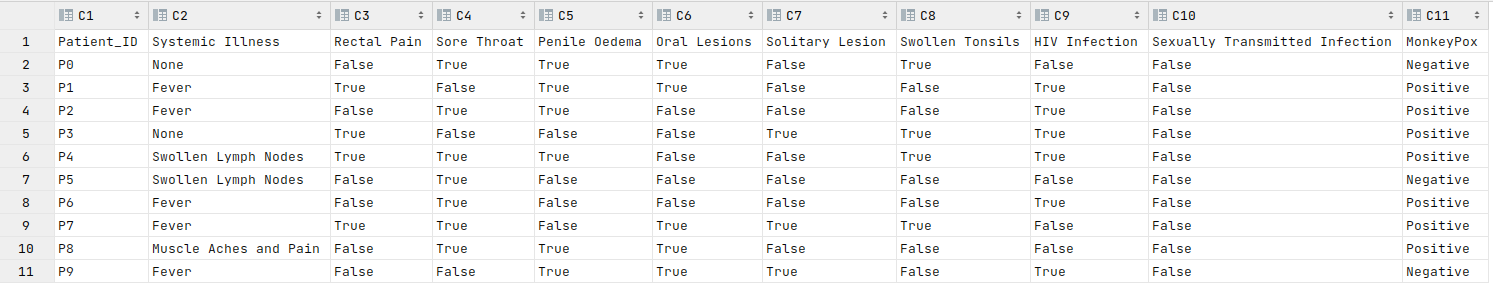
\includegraphics[width=0.8\linewidth]{Bilder/data_table.png}
		\captionof{figure}[Ausschnitt aus dem vorliegendem Datensatz]{Ausschnitt aus dem vorliegendem Datensatz}
		\label{fig:data_table}
	\end{figure}

Bei den Werten der Features handelt es sich zu einem großen Teil um \textit{bool}-Werte. Die Spalte \textit{Systemic\textunderscore Illness} stellt dabei eine Ausnahme dar. In dieser werden
vier \textit{str}-Werte verwendet: \textit{None}, \textit{Fever}, \textit{Swollen Lymph Nodes} und \textit{Muscel Aches and Pain}. Es gilt diese Werte in \textit{int}-Werte umzuwandeln. So wird \textit{None} zu 1,
\textit{Fever} zu 2, \textit{Swollen Lymph Nodes} zu 3 und \textit{Muscle Aches and Pain} zu 4. Die Spalte \textit{MonkeyPox} enthält die Werte \textit{Positive} und \textit{Negative} und gibt
an, ob der entsprechende Patient an Affenpocken erkrankt ist.

Die Werteverteilung der Features, die \textit{bool}-Werte enthalten, ist in dieser Tabelle aufgelistet: 
	
	\begin{singlespace}
	\begin{table}[H]
		\begin{adjustbox}{width=1\textwidth}
			\small
		\begin{tabular}{|l|l|l|l|l|l|l|l|l|}
			\hline  & \url{Rectal_Pain}&  \url{Sore_Throat}	& \url{Penile_Oedema} & \url{Oral_Lesion} & \url{Solitary_Lesion} &\url{Swollen_Tonsils} & \url{HIV_Infection} & \url{STI} \\
			\hline True & 12345 & 12554 & 12612 & 12486 & 12527 & 12533 & 12584  & 12446 \\
			\hline False & 12655 & 12446 & 12388& 12514 & 12473 & 12467 & 12416 & 12554\\
			\hline
		\end{tabular}
	\end{adjustbox}
		\caption{Werteverteilung der \textit{bool}-Features} %Hinzufügen einer Tabellenbeschriftung
		\label{tab:werteverteilung_features}
	\end{table}
\end{singlespace}
	

Es lässt sich feststellen, dass die Werteverteilung innerhalb der \textit{bool}-Features sehr gleichmäßig ist. 
In Bezug auf das Feature \textit{SystemicIllness}, welches ausschließlich \textit{str}-Werte enthält, lässt sich die 
Werteverteilung, durch dieses Diagramm visualisieren: 

	\begin{figure}[H]
		\centering
		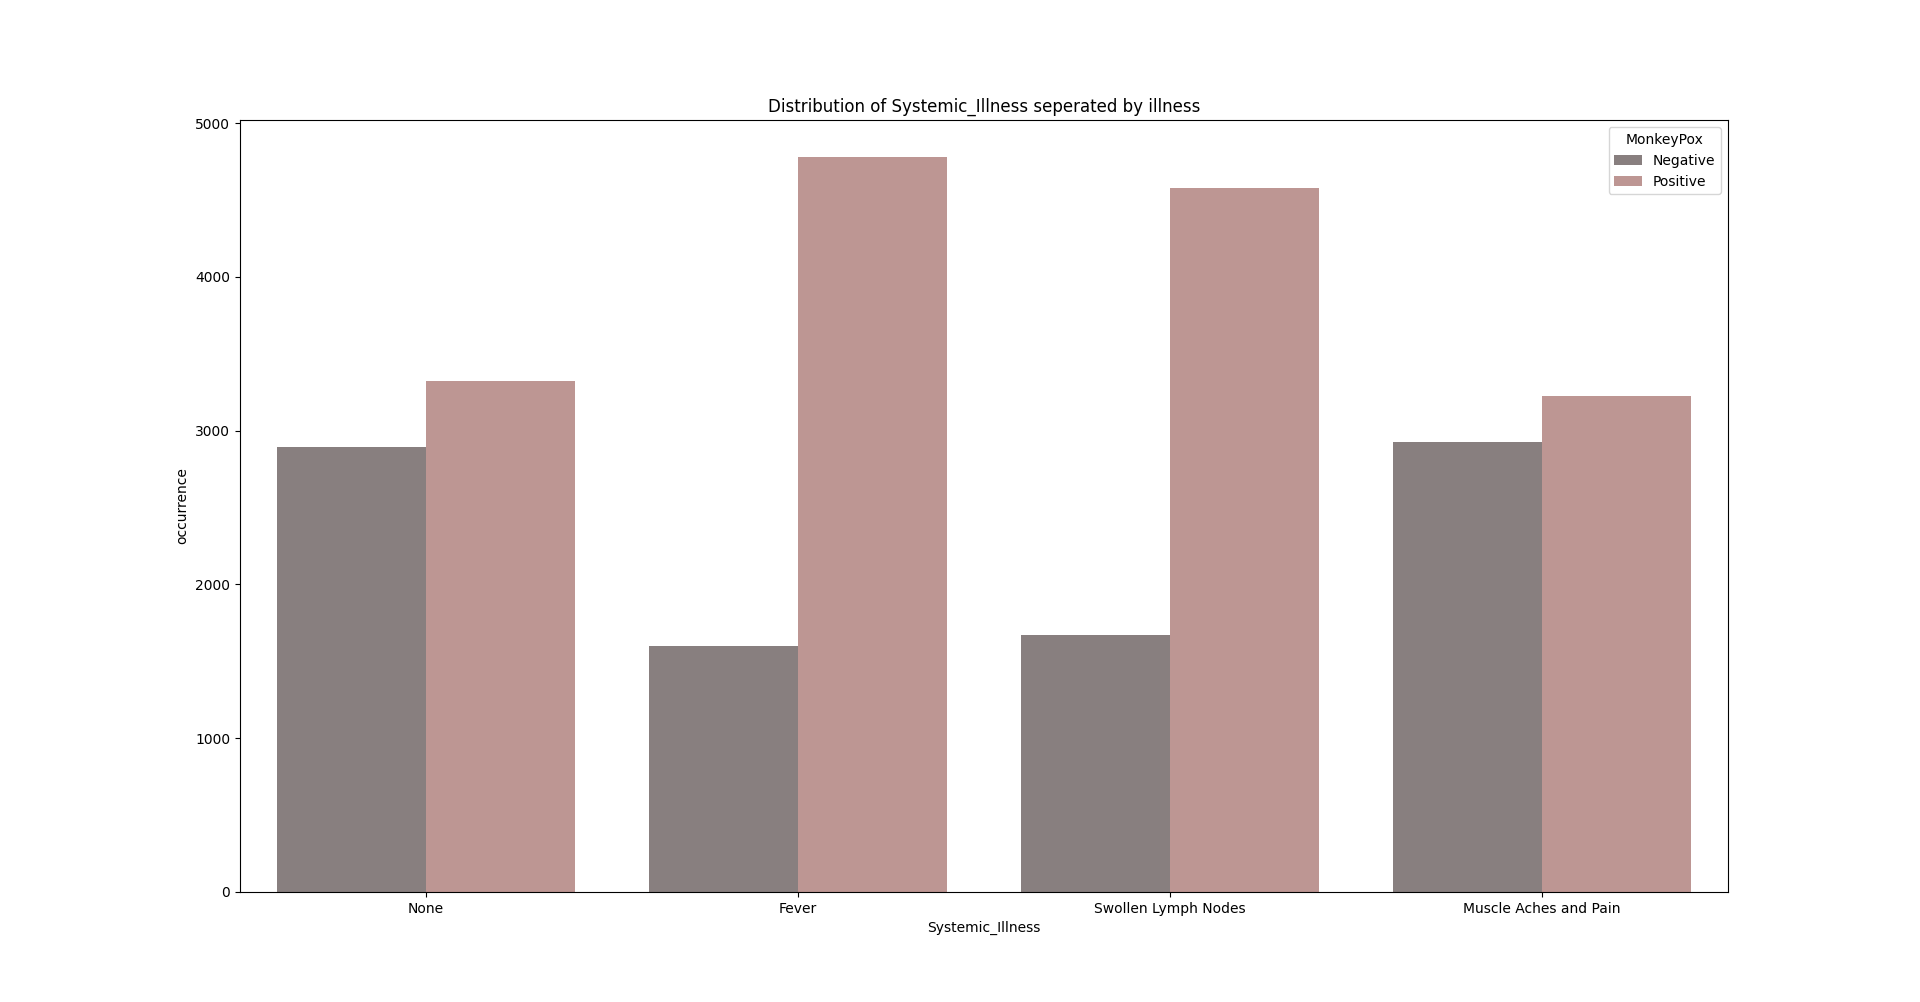
\includegraphics[width=0.8\linewidth]{Bilder/systemic_illness_plot.png}
		\captionof{figure}[Werteverteilung des Features \textit{Systemic\textunderscore Illness}]{Werteverteilung des Features \textit{Systemic\textunderscore Illness}}
		\label{fig:systemic_illness_plot}
	\end{figure}

Man stellt also fest, dass Patienten, die an \textit{Fever} oder \textit{Swollen\textunderscore Lymph\textunderscore Nodes} leiden, zu einer
höheren Wahrscheinlichkeit an Affenpocken erkranken, als Patienten, die an keiner Symptomatik (\textit{None}) oder an \textit{Muscle Aches and Pain} leiden.

In Betracht auf die Spalte \textit{MonkeyPox} lässt sich sagen, dass 15909 Patienten an Affenpocken erkrankt sind, während 9091 \textit{Negative} sind.
Diese Werteverteilung würde sich visuell folgendermaßen äußern:

	\begin{figure}[H]
		\centering
		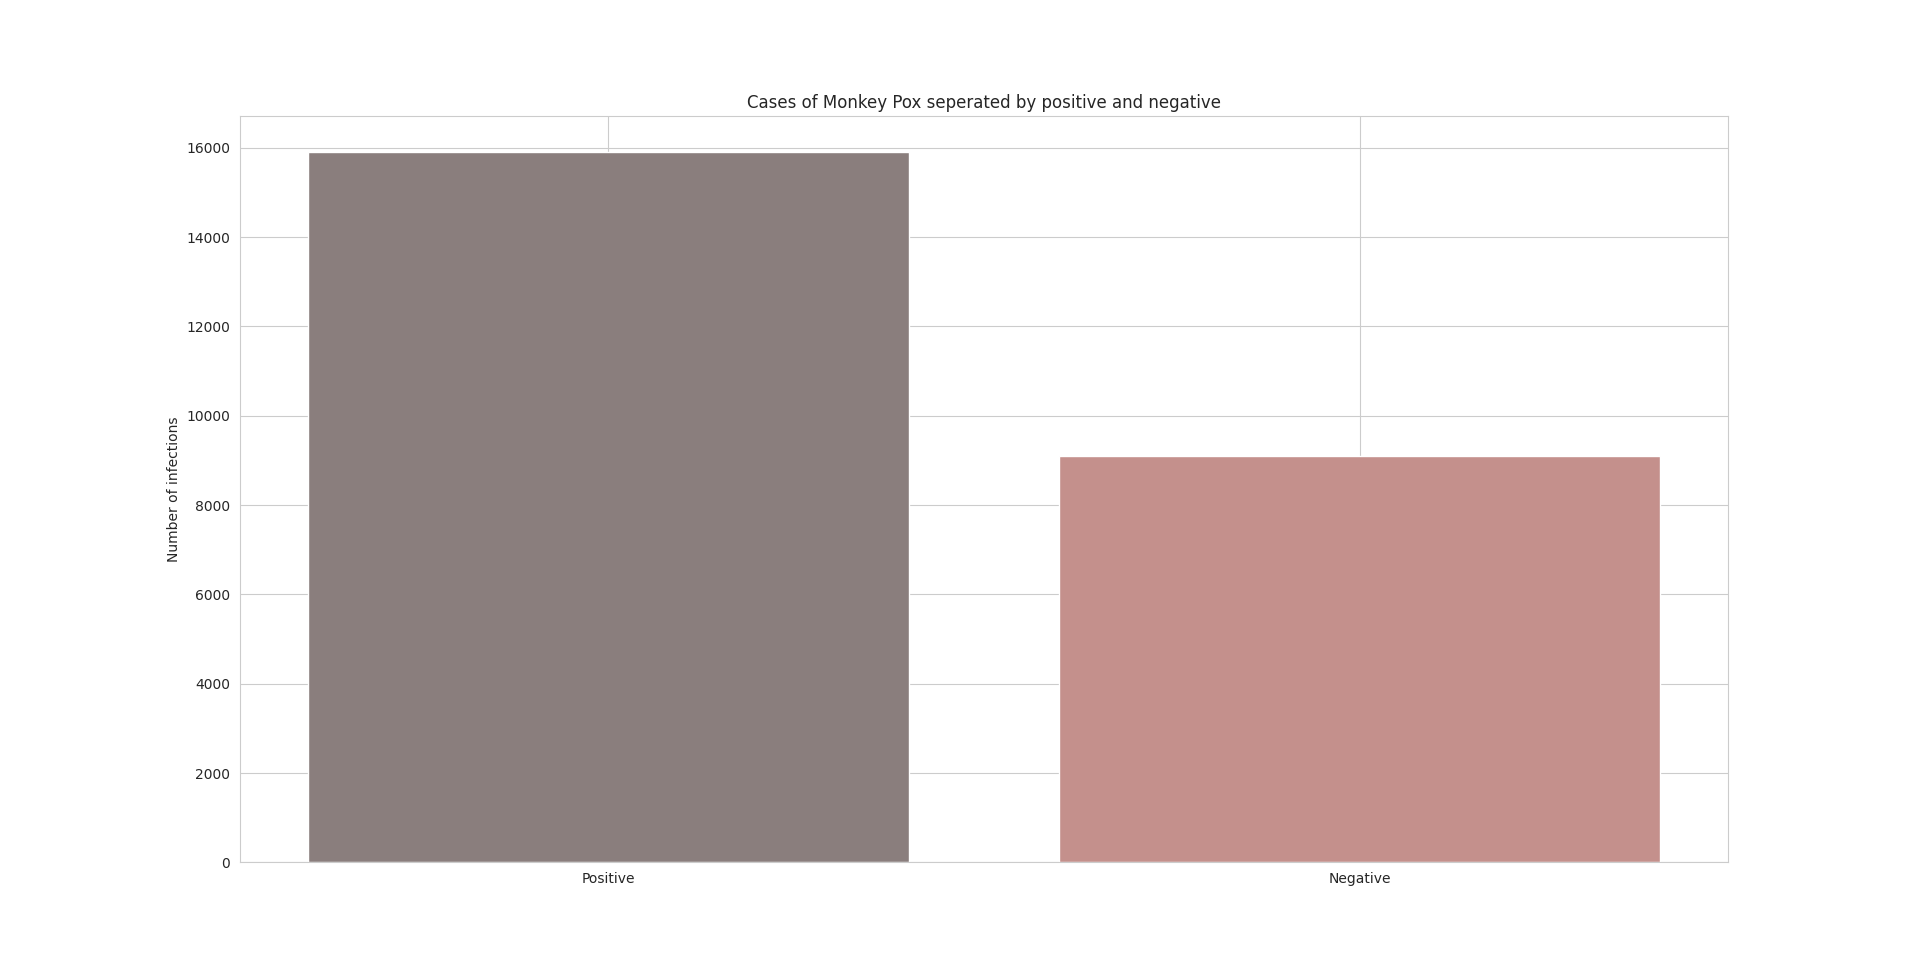
\includegraphics[width=0.8\linewidth]{Bilder/monkey_pox_plot.png}
		\captionof{figure}[Werteverteilung der Ergebnis-Spalte \textit{MonkeyPox}]{Werteverteilung der Ergebnis-Spalte \textit{MonkeyPox}}
		\label{fig:monkey_pox_plot}
	\end{figure}

	\subsection{Korrelationsanalyse}
		\label{ch:korrleations_analyse}

Zur Prüfung, ob Zusammenhänge zwischen den einzelnen Features bestehen wird eine Heatmap verwendet. 
Eine Heatmap ist eine Zusammenstellung von Rechtecken. Sie kann genutzt werden, um Muster und Veränderungen im
Zeitverlauf zu betrachten. Die x-Achse wird oft mit einem Zeitmaß bezeichnet. Die y-Achse stellt eine Variable dar, 
die die Kategorie in den Daten definiert. In Betracht auf den vorliegenden Datensatz ergibt sich die folgende Heatmap:

	\begin{figure}[H]
		\centering
		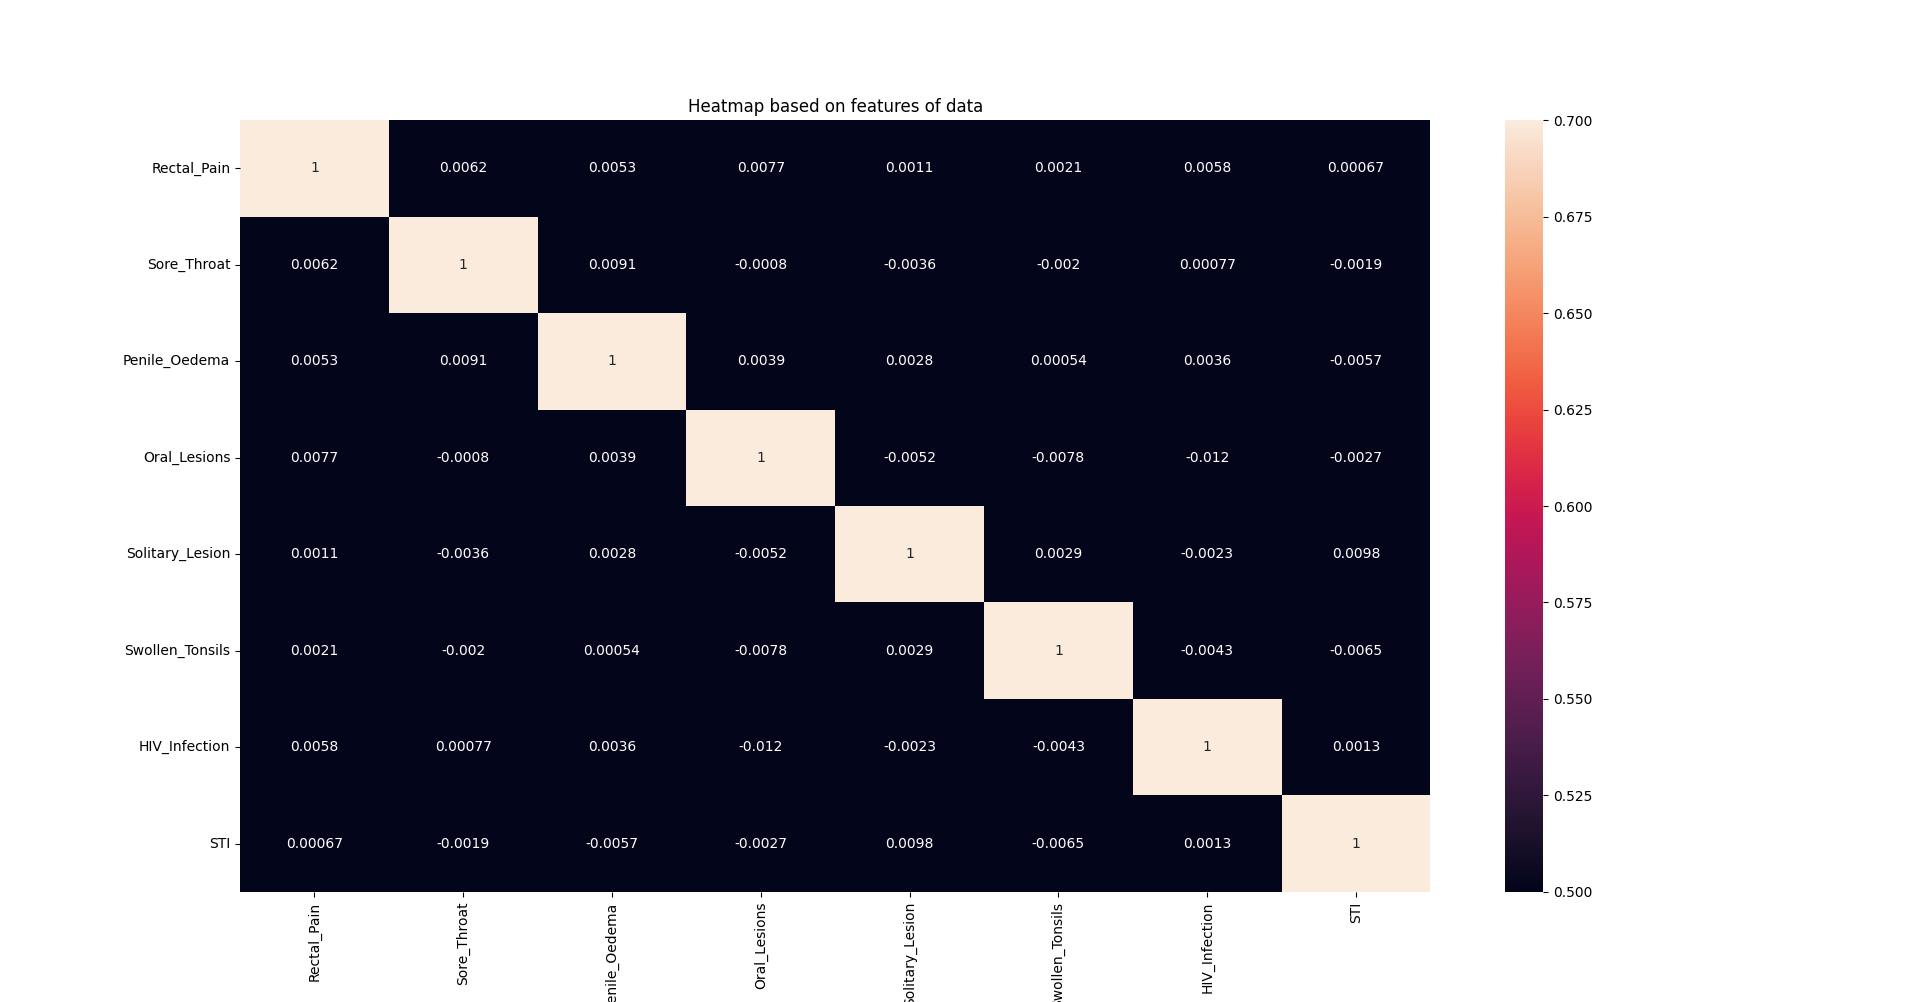
\includegraphics[width=0.8\linewidth]{Bilder/heat_map.png}
		\captionof{figure}[Aus den Features resultierende Heatmap]{Aus den Features resultierende Heatmap}
		\label{fig:heatmap}
	\end{figure}
	
Anhand von Abbildung \ref{fig:heatmap} lässt sich also feststellen, dass die berechneten Wahrscheinlichkeiten sich in einem sehr kleinem beziehungsweise 
negativen Bereich befinden. Es bestehen somit keine Zusammenhänge und Korrelationen zwischen den verschiedenen Features. 

Ein weiterer Schritt in der Korrelationsanalyse stellt die Betrachtung der Lift und Konfidenz Werte dar. Dabei ist es notwendig, den 
Datensatz in so weit zu bearbeiten, dass die verschiedenen Werte von \textit{Systemic\textunderscore Illness}, als eigene Spalten betrachtet werden. 
Dies ist gefordert, da die verschiedenen Krankheisbilder der Spalte \textit{Systemic\textunderscore Illness} als eigene Symptome (Features) verstanden werden sollen und somit mehrere Feature-Kombinationen 
getestet werden können. Demnach sieht der überarbeitete Datensatz folgendermaßen aus: 

	\begin{figure}[H]
		\centering
		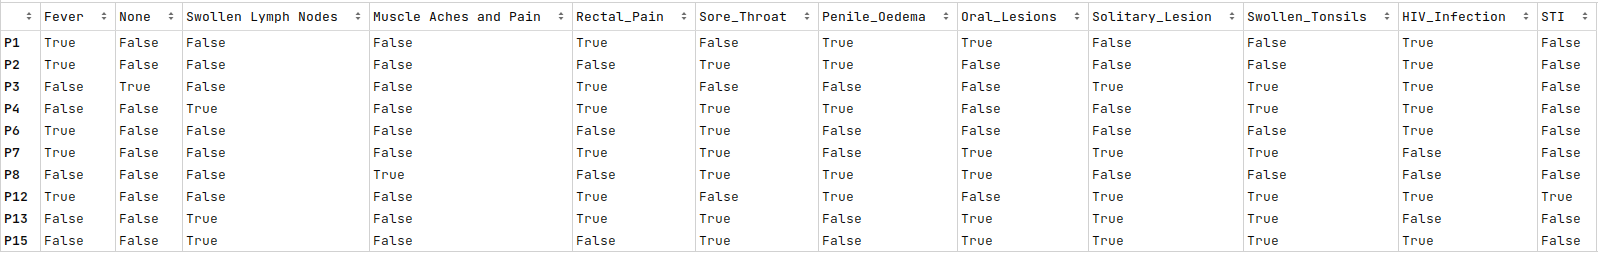
\includegraphics[width=0.8\linewidth]{Bilder/tranp_df.png}
		\captionof{figure}[Ausschnitt des erweiterten Datensatzes]{Ausschnitt des erweiterten Datensatzes}
		\label{fig:transp_feature}
	\end{figure}

Die Analyse dieser Werte stützt die gesammelten Erkenntnisse aus der Heatmap. Die maximale Konfidenz ist 0.604167, der entsprechende Lift
1.104538. Dementsprechend ist festzustellen, dass die Werte sich gegenseitig wenig bis gar nicht beeinflussen beziehungsweise nicht zusammenhängen. 


	\section{Genauigkeitsanalyse}
		\label{ch:genauigkeit_analyse}

In diesem Kapitel werden verschiedene Genauigkeiten mit mehreren Modellen und Feature-Kombinationen ermittelt. Dabei wird versucht, die best mögliche Genauigkeit herauszufinden. 
Danach wird das ausgewählte Modell grafisch auf Overfitting überprüft.  

	\subsection{Wahl des Modells}
		\label{ch:wahl_modell}

Zum Einen wird eine Untersuchung mit Bayes (\textit{GaussianNB()}) getätigt. Im Laufe der Untersuchung wird der Zufallsstrom nicht aktiv vorgegeben, diese also vom Moll selber gewählt.
67.82 ist dabei die berechnete Genauigkeit. Die ermittelte Genauigkeit in diesem Modell stellt sich als wenig zufriedenstellen heraus. Es ergibt sich somit die Frage,
ob sich diese optimieren lässt.

In der Datei \textit{utils.py} wird eine Funktion \textit{create\textunderscore feature\textunderscore accuracy\textunderscore dict()} entwickelt, bei welcher jede mögliche Feature-Kombination für drei Modellen angewendet wird. 
Bei den drei Modellen handelt es sich um  \textit{DecisionTreeClasifier()}, \textit{RandomForestClassifier()} und \textit{GaussianNB()}. Die Feature-Kombinationen, das verwendete Modell (Key) und die korrespondierenden Genauigkeiten (Value) werden in 
einer Dictionary gespeichert. Diese Dictionary lässt sich anhand der Genauigkeit absteigend sortieren. Man kommt zu dem Ergebnis, dass für das Modell \textit{RandomForestClassifier} und 
den Features: \textit{Systemic\textunderscore  Illness}, \textit{Rectal\textunderscore Pain}, \textit{Sore\textunderscore Throat}, \textit{Solitary\textunderscore Lesion}, \textit{HIV\textunderscore Infection} und \textit{STI} 
eine Genauigkeit von 69.71 berechnet wird.  

	\lstinputlisting[label=lst:plot, captionpos=b,caption=Verwendetes Modell Feature-Kombination und korrespondierende Genauigkeitst]{Listing/dict.txt}


In Bezug auf Listing \ref{lst:plot} stellt man fest, dass die oben gennante Feature-Kombination von den perfomantesten Modellen verwendet wird.
Diese Untersuchung ermöglicht es, die Genauigkeit um 1\% zu optimieren und \textit{RandomForestClassifier} als das beste Modell für diesen Datensatz zu erkennen.  

	\subsection{Prüfung auf Overfitting}
		\label{ch:pruefung_overfitting}

Aufbauend auf Kapitel \ref{ch:wahl_modell} ist es wichtig festzustellen, ob beziehungsweise wann Overfitting in \textit{RandomForestclassifier()} auftritt. Overfitting beschreibt das Phänomen, dass
sich Daten zu sehr den Trainingsdaten anpassen. Hierbei besteht die Gefahr, dass der Algorithmus den Datensatz auswendig, aber nicht die zugrundeliegenden Muster und Zusammenhänge erkennt.

Um Overfitting in dem vorliegenden Datensatz zu erkennen wird in der \textit{utils.py} eine weitere Funktion \textit{check\textunderscore over\textunderscore fitting} hinzugefügt. In welcher
die Genauigkeit anhand der berechneten Test- und Trainingsdaten und dem ausgewählten Modell (\textit{RandomForestClassifier}) aus 
Kapitel \ref{ch:wahl_modell} für die Baumtiefen 2 bis 21 berechnet wird. Die Test- und Trainingsdaten werden dabei im Verhältnis 50:50 geteilt. 
Das Ergebnis dieser Untersuchung wird grafisch in Form eines Plots ausgewertet: 

	\begin{figure}[H]
		\centering
		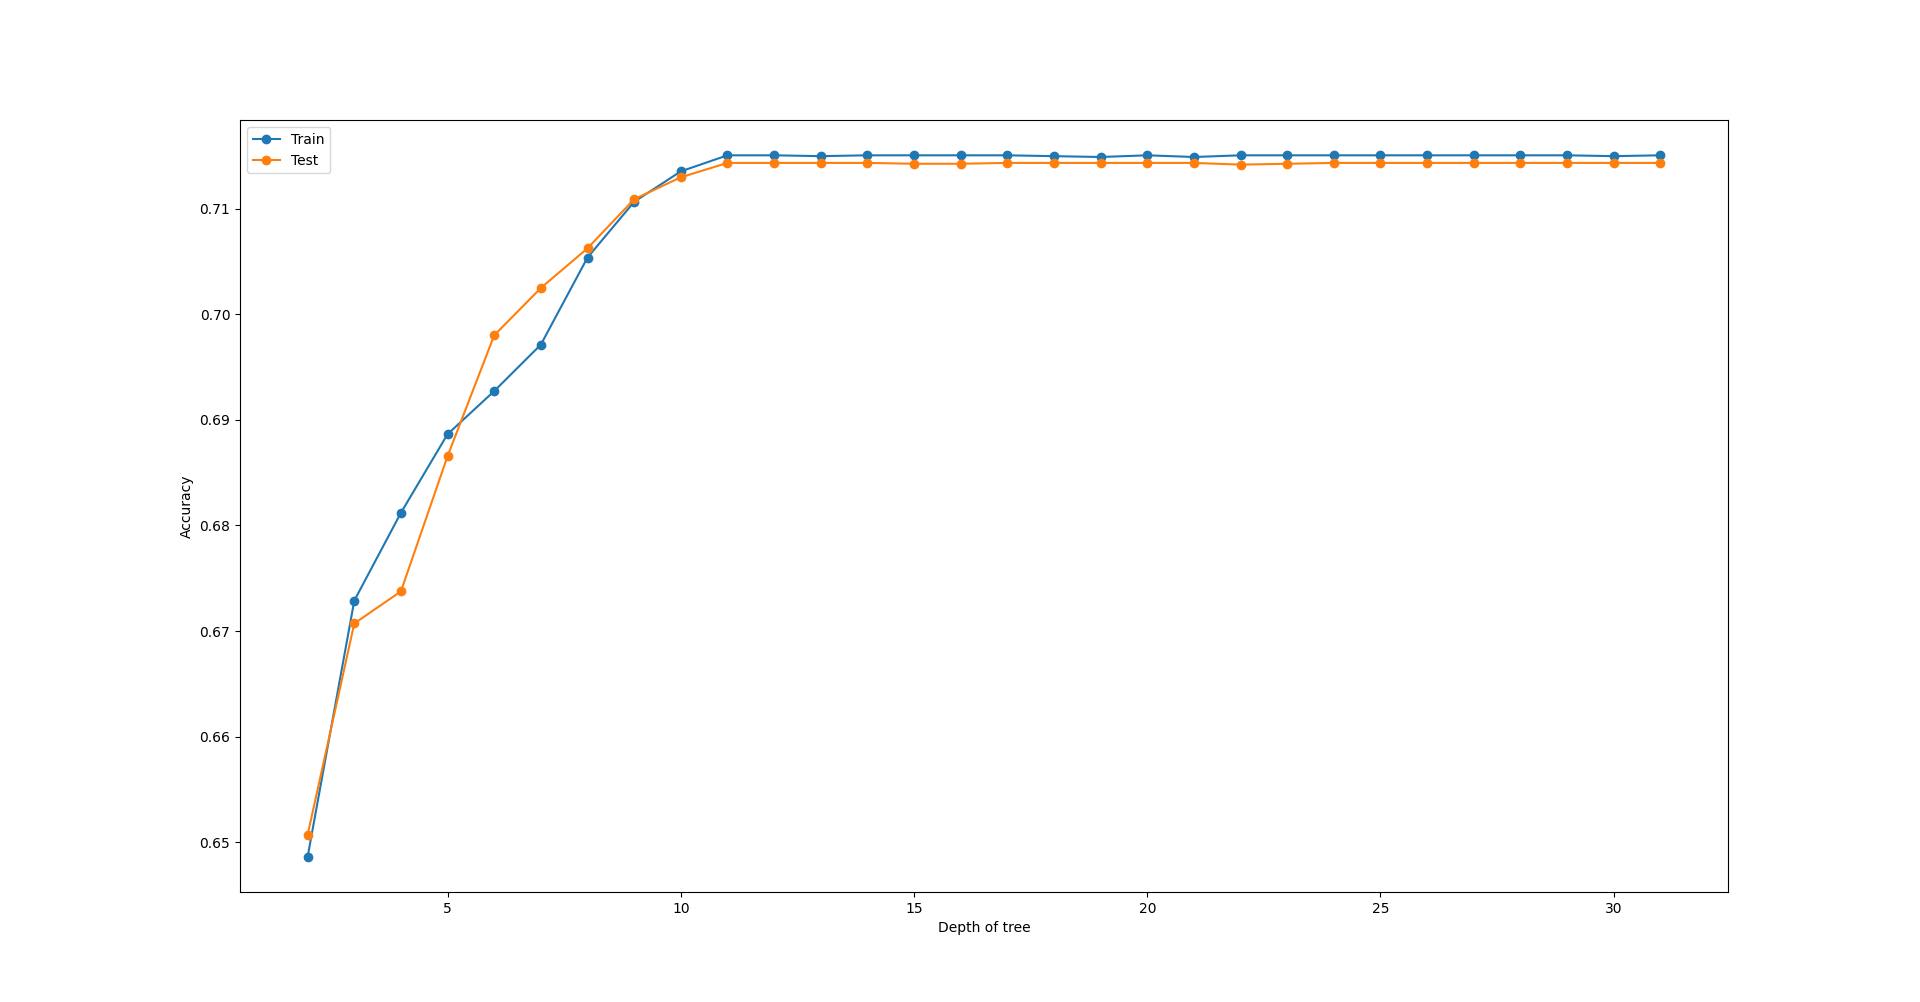
\includegraphics[width=0.8\linewidth]{Bilder/overfitting_plot.png}
		\captionof{figure}[Genauigkeits-Verlauf der Test- und Trainingsdaten bei steigender Baumtiefe]{Genauigkeits-Verlauf der Test- und Trainingsdaten bei steigender Baumtiefe}
		\label{fig:overfitting}
	\end{figure}

Bei Betrachtung von Abbildung \ref{fig:overfitting} stellt man fest, dass ab einer Baumtiefe von 11, die Test- und Trainingsdaten parallel 
verlaufen. Dieses Verhalten ist zwar kein Indiz für Overfitting. Es ist ein eher ein Zeichen dafür, dass sich die Test- und Trainingsdaten aber einer
Baumtiefe von 11 stabilisieren. Demnach sollte die maximale Tiefe des Baumes in \textit{RandomForestClassifier} mit Hilfe der Variable \textit{max\textunderscore depth} 
auf 11 festgelegt werden.  
 


	\subsection{Darstellung als Entscheidungsbaum}
		\label{ch:entscheidungsbaum}

Das Aufzeigen eines Entscheidungsbaums wird gewählt, um anhand von verschiedenen visualisierten Antwortoptionen auf eine Affenpocken-Erkrankung zu schließen.
Da es sich in dieser Studienarbeit, um einen sehr großen Datensatz handelt, ist es notwendig den Entscheidungsbaum durch den Parameter \textit{min\textunderscore sample\textunderscore split}
etwas zu kürzen. Dieser wird in der folgenden Abbildung auf 0.2 gesetzt. 

	\begin{figure}[H]
		\centering
		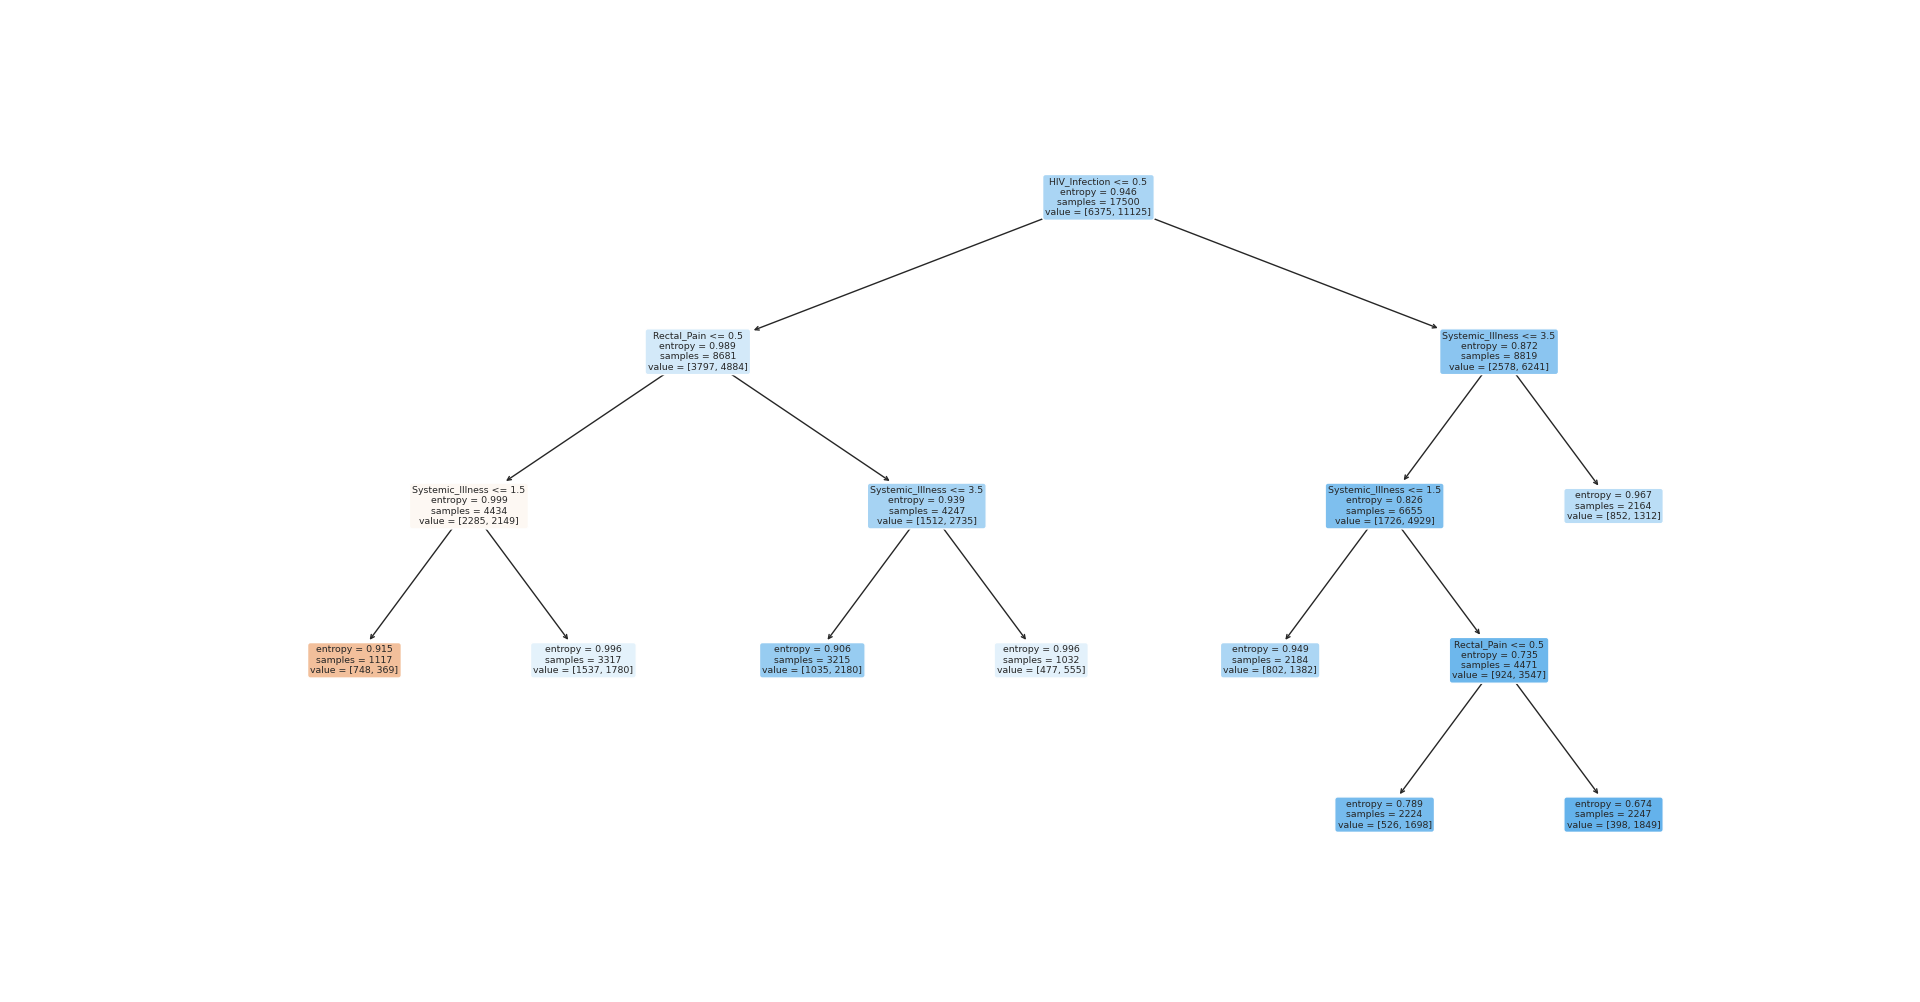
\includegraphics[width=0.8\linewidth]{Bilder/decision_tree.png}
		\captionof{figure}[Gekürzter Entscheidungsbaum]{Gekürzter Entscheidungsbaum}
		\label{fig:decisiontree}
	\end{figure}

Es lässt sich also sagen, dass die True- und False-Werte, der Endknoten zu nahe beieinander liegen, um eine klare Aussage zu treffen. 
Demnach lässt sich anhand des Baumes schwer ein Muster ablesen beziehungsweise nicht auf eine Affenpocken-Erkrankung schließen.  

	\section{Erstellung eines neuronalen Netzes}
		\label{ch:neuronlaes_netz}

Am Ende der Datenanalyse wird ein neuronales Netz erstellt. Der erste Schritt besteht darin, die Daten für die Arbeit mit 
\textit{tensorflow} vorzubereiten. Hierbei werden die enthaltenen \textit{bool}- und \textit{int}-Werte in 
\textit{float}-Werte umgewandelt. Dies wird durch die Funktion \textit{prepare\textunderscore for\textunderscore tensor}
in der \textit{utils.py} Datei bewärkstelligt. Auf Funktionen der Bibliothek \textit{sklearn.preprocessing} wie 
beispielsweise \textit{MinMaxScaler} konnte aufgrund des einheitlichen sowie kleinen Wertebereichs verzichtet werden. 

Der zweite Schritt, besteht in der Definition des neuronalen Netzes, dieses ist folgendermaßen aufgebaut:

	\lstinputlisting[label=lst:neuronal_network, captionpos=b,caption=Code des neuronalen Netzes]{Listing/neuronal_network.py}

In Listing \ref{lst:neuronal_network} werden für den Aufbau des Netzes insgesamt 5
Schichten verwendet. Je eine \textit{input}- sowie \textit{output}-Schicht. Aufgrund der 
Größe des Datensatzes werden 3 versteckte Schichten verwendet.
Die Anzahl der Neuronen innerhalb der versteckten Schichten ist auf 15 festgelegt, bei der \textit{input}-
Schicht liegt sie bei 9. Die verwendeten Aktivierungsfunktionen beschränken sich auf \textit{relu} und 
\textit{sigmoid}. Die Verlustfunktion \textit{mse} hat sich im Laufe dieser Untersuchung als die beste Wahl herausgestellt.

Es ergibt sich somit eine berechnete Genauigkeit von 0.69 und ein Verlust von 0.20. Graphisch sieht der Epochenverlauf der Verlust- und 
Genauigkeitswerte folgendermaßen aus: 

	\begin{figure}[H]
		\centering
		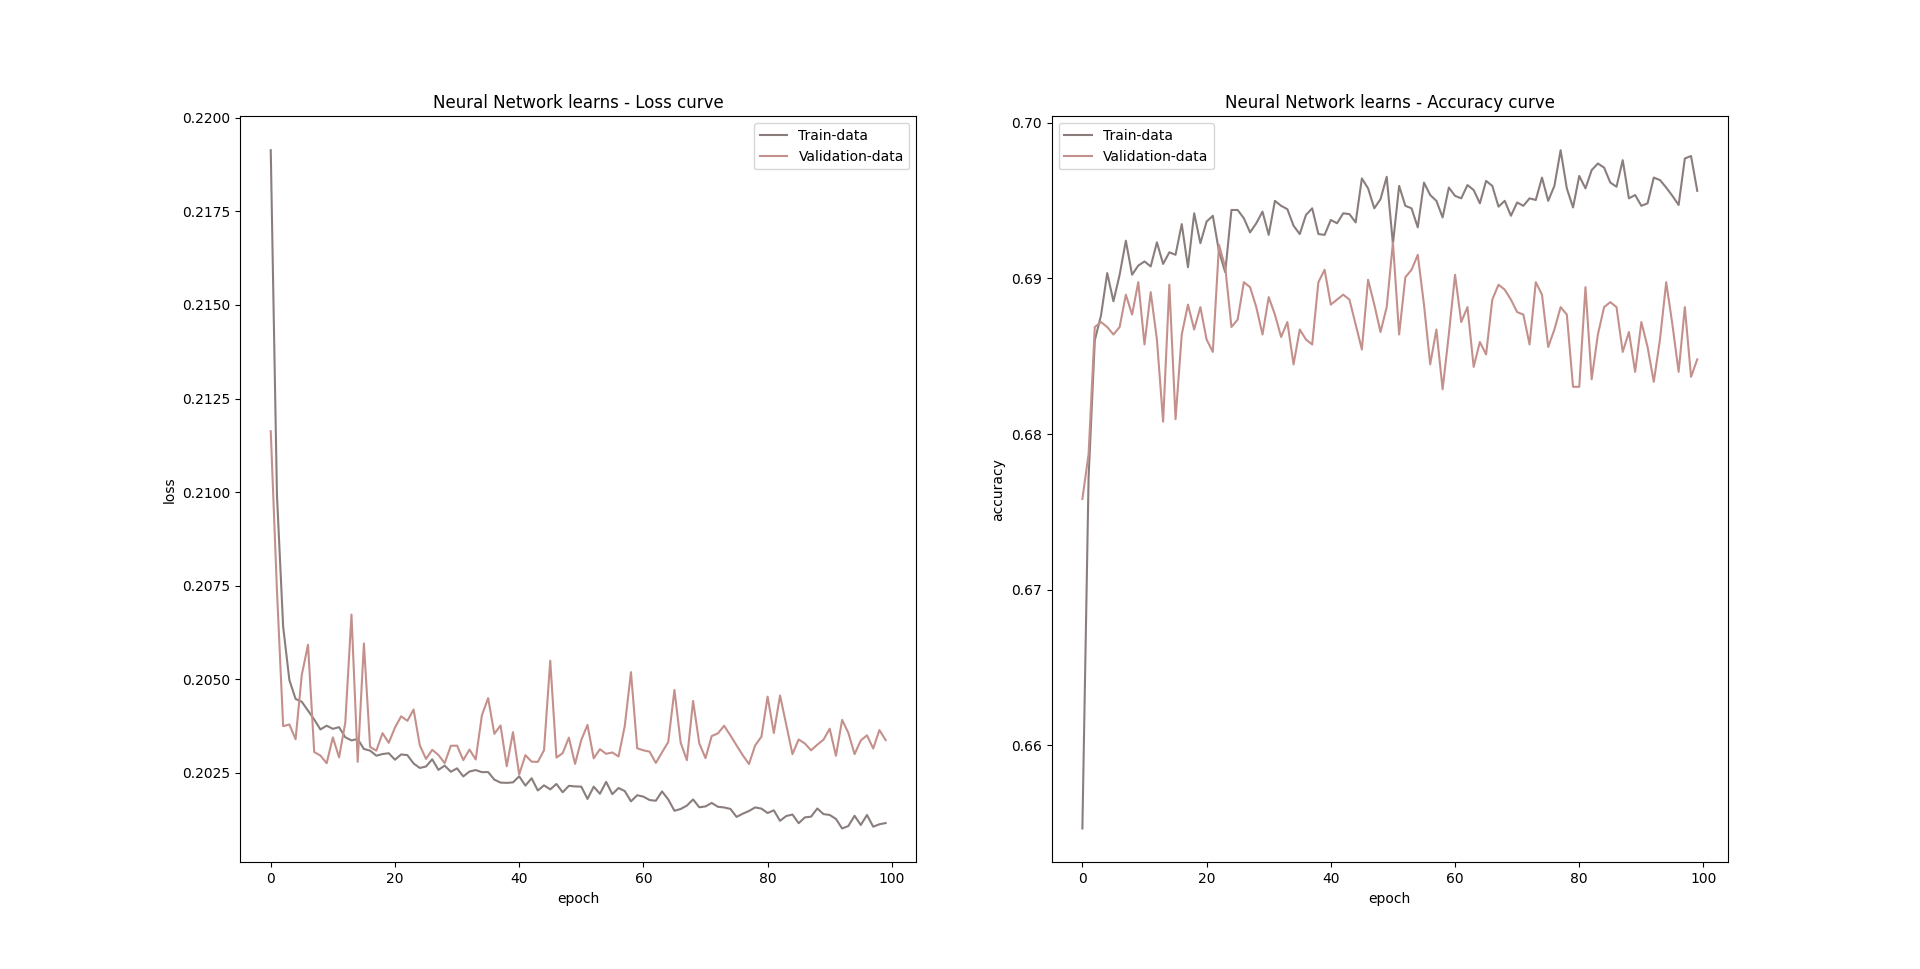
\includegraphics[width=0.8\linewidth]{Bilder/neural_network.png}
		\captionof{figure}[Verlust- und Genauigkeitskurven des neuronalen Netzes]{Verlust- und Genauigkeitskurven des neuronalen Netzes}
		\label{fig:neural_network}
	\end{figure}

Es ist ein Abfall im Verlust der Test- und Trainingsdaten zu verzeichnen. Der Verlust der Trainingsdaten ist jedoch stärker. 
In Bezug auf die Testdaten ist anstelle eines Abfalls, eher eine Schwankung erkennbar. Der ermittelte Genauigkeitsverlauf
der Trainings- und Testdaten schwankt zwar, ist aber insgesamt stabil. Somit ist in Betracht der Verlust- und Genauigkeitskurven
kein Overfitting zu verzeichnen. 


	\section{Bewertung der Ergebnisse}
		\label{ch:bewertungs_ergebnisse}

Nach einer ausgiebigen Analyse des vorliegenden Datensatzes können keine eindeutigen Schlüsse aus diesem Datensatz gezogen werden.
Man kann weder anhand eines bestimmten Features auf eine Affenpocken-Erkrankung schließen, noch besteht ein Zusammenhang/ Korrelationen
zwischen den Features. Die Datenanalyse mithilfe verschiedener Modelle blieb ebenfalls erfolglos, so konnte anhand verschiedener 
Feature-Kombinationen und dem Modell \textit{RandomForestClassifier} nur eine Genauigkeit von $\approx 0.70$ ermittelt werden. 
Die ermittelte Genauigkeit lässt vermuten, dass der vorliegende Datensatz für medizinische Untersuchungen zu gering ist. 
Overfitting konnte im verwendeten Modell \textit{RandomForestClassifier()} als auch im \textit{Neuronalen Netz} nicht nachgewiesen werden. 

Der Grund für diese eher erfolglose Datenanalyse liegt vermutlich an der Homogenität der Daten. 
In Kapitel \ref{ch:genauigkeit_analyse} wurde bereits bewiesen, dass kein Feature ein wirkliches Indiz für eine 
Affenpocken-Erkrankung darstellt. Es wäre sinnvoller gewesen, den Features \textit{int}-Werte beispielsweise in einem Intervall [0, 5] 
zu geben. Dabei beschreiben die Werte des Intervalls die Heftigkeit der jeweiligen Symptomatik.


		\pagebreak
		%-------------------------------------------------------------------------------------
		% Verzeichnisse %-------------------------------------------------------------------------------------
		\rhead{Verzeichnisse} %Kopftextbeschriftung

		\stepcounter{section}
		\phantomsection \label{Verzeichnisse}
		\addcontentsline{toc}{section}{Verzeichnisse} %Ohne Nummer ins Inhaltsverzeichnis
		\renewcommand{\thesection}{\Roman{verzeichnis}}
		\section*{Verzeichnisse} 
		\rhead{Verzeichnisse}

		% Abbildungsverzeichnis
		\listoffigures
		\pagebreak

		% Tabellenverzeichnis
		\stepcounter{verzeichnis}
		\listoftables
		\pagebreak

		\stepcounter{verzeichnis}
        \lstlistoflistings
        \pagebreak

\vspace{-3em}


    
\pagebreak

	\end{document}
